\fancypagestyle{brandtitle}{%
\fancyhf{}
\fancyhead[L]{\raisebox{-7pt}{
\includegraphics[height=21pt]{assets/rockmatrix.png}}\hspace{5pt}\raisebox{-4pt}{{\sffamily\bfseries\fontsize{9}{10}\selectfont\shortstack[l]{ROCK\\[-1pt]MATRIX}}}}
\fancyfoot[C]{\thepage}
\renewcommand{\headrulewidth}{0.3pt}
\renewcommand{\headruleskip}{2pt}
}
\thispagestyle{brandtitle}
\begin{center}
{\LARGE\bfseries EdgeRock: Strong Reasoning at Constant Memory\par}
\vspace{12pt}
\begingroup
\hypersetup{urlcolor=black}
\renewcommand{\arraystretch}{1.0}
\begin{tabular*}{0.84\linewidth}{@{\extracolsep{\fill}}ccc@{}}
Huishan Ji & Weiming Zhang & Qirui Ye \\
{\small\href{mailto:jihs@stonehill-tech.com}{jihs@stonehill-tech.com}} &
{\small\href{mailto:zhangwm@stonehill-tech.com}{zhangwm@stonehill-tech.com}} &
{\small\href{mailto:qiruiy@andrew.cmu.edu}{qiruiy@andrew.cmu.edu}} \\[5pt]
Jinchao Xu & Yike Guo & Hua Xu\textsuperscript{*} \\
{\small\href{mailto:jinchao.xu@kaust.edu.sa}{jinchao.xu@kaust.edu.sa}} &
{\small\href{mailto:yikeguo@ust.hk}{yikeguo@ust.hk}} &
{\small\href{mailto:huaxu@ust.hk}{huaxu@ust.hk}}
\end{tabular*}
\endgroup
\par\vspace{8pt}
{\sffamily\footnotesize
\href{https://github.com/rockmatrix-ai/EdgeRock}{\raisebox{-2.2pt}{
\includegraphics[height=10pt]{assets/github.pdf}}\hspace{5pt}github.com/rockmatrix-ai/EdgeRock}\hspace{2.2em}
\href{https://huggingface.co/rockmatrix-ai/EdgeRock}{\raisebox{-2.2pt}{
\includegraphics[height=10pt]{assets/huggingface.pdf}}\hspace{5pt}huggingface.co/rockmatrix-ai/EdgeRock}\par}
\end{center}
\begingroup
\renewcommand{\thefootnote}{\fnsymbol{footnote}}
\footnotetext[1]{Corresponding author.}
\endgroup
\begin{abstract}
We present EdgeRock, a family of multimodal models that deliver strong reasoning at constant memory. As \mbox{reasoning} trajectories lengthen, growing \mbox{key--value} (KV) caches consume accelerator memory, limit serving concurrency, and compete with perception and control on edge devices. Keeping history fixed makes its memory demand predictable as reasoning continues. Constant memory alone is not new. Recurrent, state-space, and sliding-window models already bound history, but preserving direct access to distant details remains a challenge. EdgeRock combines recurrent state and local attention with \emph{Rock Memory Anchors} (RMA): learned KV records held in a fixed-size bank and directly retrievable long after their source leaves the window. EdgeRock-4B, our first open-source release, supports text and image reasoning and reaches 82.9\% mean pass@1 on AIME 2024--2026, compared with at most 18.8\% among the bounded-state models we evaluate, including 14B-class models. This brings reasoning at constant memory into the range of leading compact models. Relative to its source backbone, EdgeRock-4B reduces attention KV storage by up to 99.1\% and delivers up to 5.65$\times$ higher end-to-end batch throughput.
\end{abstract}
\begin{figure}[!ht]
\centering
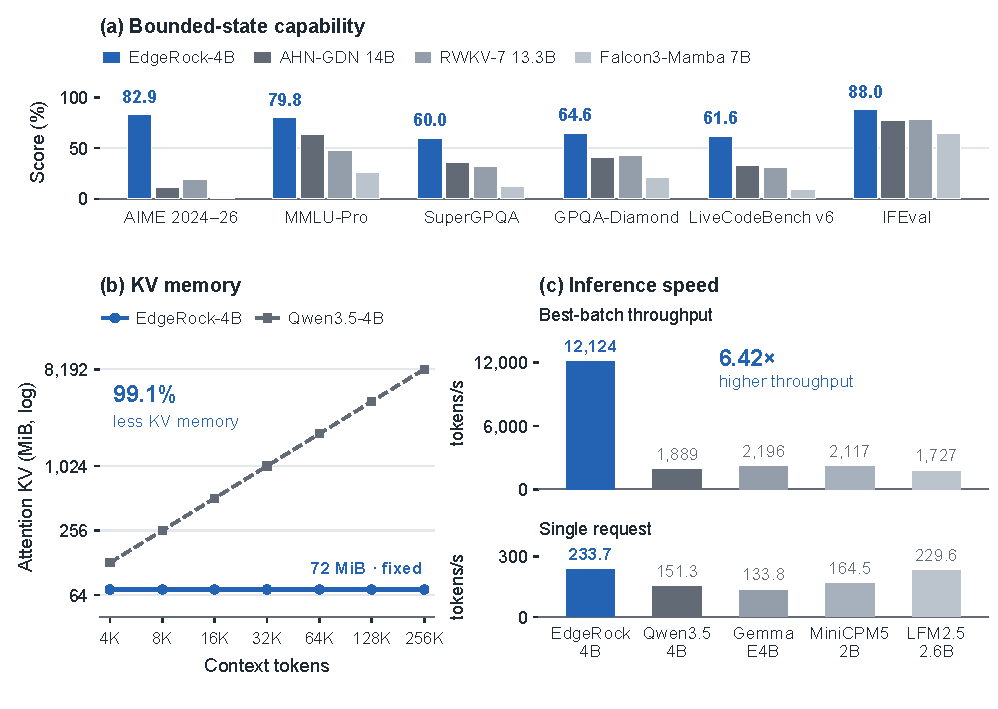
\includegraphics[width=0.96\linewidth]{hero_capability.pdf}
\caption{\textbf{Reasoning at constant memory.} \textbf{(a)} EdgeRock-4B leads the displayed 7B--14B bounded-state models on six text metrics; AIME averages 2024--2026 equally. \textbf{(b)} Configuration-derived BF16 attention KV capacity per sequence (log axes). EdgeRock uses 72\,MiB, 99.1\% less than Qwen3.5-4B at 256K. \textbf{(c)} Top: output-token throughput for 32K input and 32K output with repeated prompts, including prefill time, at each model's best measured batch (Appendix Table~\ref{tab:peer-throughput}); EdgeRock achieves 5.65$\times$ Qwen3.5-4B's throughput. Bottom: cumulative decode rate for 128K input and 128K output at batch size 1. All runs use BF16 weights and KV on one Hopper 80GB GPU.}
\label{fig:overview}
\end{figure}
\clearpage
